\setAuthor{Richard Luhtaru}
\setRound{piirkonnavoor}
\setYear{2023}
\setNumber{G 1}
\setDifficulty{1}
\setTopic{TODO}

\prob{Valgusvihk}
Maril on taskulamp, millest väljub paralleelne valgusvihk diameetriga $\SI{30}{\mm}$. Et koondada lambist tulenev valgus eredamaks, soovib Mari läätsede abil muuta valgusvihu väiksemaks paralleelseks valgusvihuks diameetriga $\SI{5}{\mm}$. Mari tuhnib oma sahtlis ringi ning leiab, et tal on nii kumer- kui nõgusläätsed järgnevate fookuskaugustega: $\SI{1}{\cm}$, $\SI{2}{\cm}$, $\SI{3}{\cm}$, $\SI{5}{\cm}$, $\SI{8}{\cm}$, $\SI{10}{\cm}$, $\SI{12}{\cm}$ ja $\SI{15}{\cm}$. Leidke, kuidas ja milliste fookuskaugustega läätsede abil on Maril võimalik oma eesmärk saavutada, kasutades
\\ (a) kaht kumerläätse.
\\ (b) üht kumerläätse ja üht nõgusläätse.
\\ Kummalgi juhul joonistage skeem.


\hint

\solu
Kummagi juhu skeemid on toodud allpool. Mõlemal juhul läätsede fookused kattuvad, mistõttu valgusvihk jääb paralleelseks pärast läätsede läbimist.

\begin{figure}[h]
    \centering
    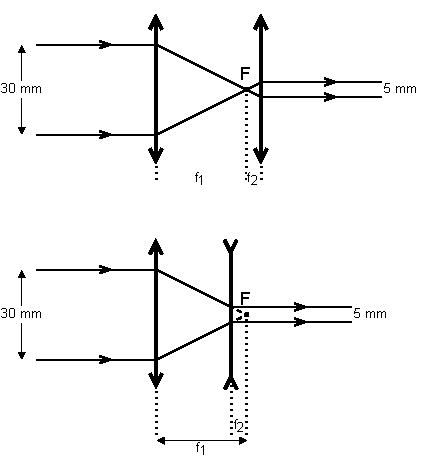
\includegraphics[width=.5\linewidth]{2023-v2g-01-sol.pdf}
\end{figure}

Sarnastest kolmnurkadest leiame, et kummalgi juhul $\frac{f_1}{f_2} = \frac{\SI{30}{mm}}{\SI{5}{mm}} = 6$. Ainsad Maril olevad läätsed, mille fookuskauguste suhe on $6$, on $\SI{12}{cm}$ ja $\SI{2}{cm}$. Seega esimesel juhul on Maril vaja kumerläätsi fookuskaugustega $\SI{12}{cm}$ ja $\SI{2}{cm}$. Teisel juhul on Maril vaja kumerläätse fookuskaugusega $\SI{12}{cm}$ ja nõgusläätse fookuskaugusega $\SI{2}{cm}$.

Tõestust, et teised läätsepaarid ei sobi, ei ole vaja.
\probend